\begin{frame}{Базовая работа с Git}{Журнал коммитов}
    \begin{columns}
        \begin{column}{0.6\textwidth}
            \begin{itemize}
                \item
                      Все созданные коммиты можно просмотреть в журнале коммитов (git log)
                \item
                      По умолчанию, будут выведены коммиты, начиная с последнего.
                \item
                    Без дополнительных настроек, будет выведена краткая информация о коммите (автор, время создания)
                \item
                      При помощи флагов можно так же сортировать и фильтровать коммиты
                      Например, git log --pretty=oneline выведет каждый коммит в отдельной строке
            \end{itemize}
        \end{column}
        \begin{column}{0.4\textwidth}
            \begin{figure}
                \centering
                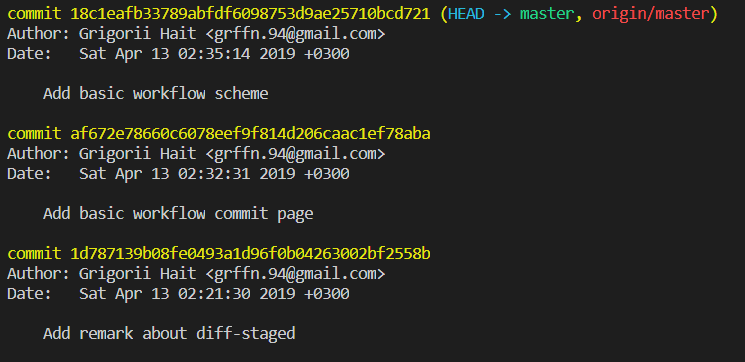
\includegraphics[width=\textwidth]{images/git-log-example.png}
                \caption{Пример git log}
            \end{figure}
        \end{column}
    \end{columns}

\end{frame}